%%%%%%%%%%%%%%%%%%%%%%%%%%%%%%%%%%%%%%%%%%%%%%%%%%%%%%%%%%%%%%%%%%%%%%%%%%%%%%%%
% Template for USENIX papers.
%
% History:
%
% - TEMPLATE for Usenix papers, specifically to meet requirements of
%   USENIX '05. originally a template for producing IEEE-format
%   articles using LaTeX. written by Matthew Ward, CS Department,
%   Worcester Polytechnic Institute. adapted by David Beazley for his
%   excellent SWIG paper in Proceedings, Tcl 96. turned into a
%   smartass generic template by De Clarke, with thanks to both the
%   above pioneers. Use at your own risk. Complaints to /dev/null.
%   Make it two column with no page numbering, default is 10 point.
%
% - Munged by Fred Douglis <douglis@research.att.com> 10/97 to
%   separate the .sty file from the LaTeX source template, so that
%   people can more easily include the .sty file into an existing
%   document. Also changed to more closely follow the style guidelines
%   as represented by the Word sample file.
%
% - Note that since 2010, USENIX does not require endnotes. If you
%   want foot of page notes, don't include the endnotes package in the
%   usepackage command, below.
% - This version uses the latex2e styles, not the very ancient 2.09
%   stuff.
%
% - Updated July 2018: Text block size changed from 6.5" to 7"
%
% - Updated Dec 2018 for ATC'19:
%
%   * Revised text to pass HotCRP's auto-formatting check, with
%     hotcrp.settings.submission_form.body_font_size=10pt, and
%     hotcrp.settings.submission_form.line_height=12pt
%
%   * Switched from \endnote-s to \footnote-s to match Usenix's policy.
%
%   * \section* => \begin{abstract} ... \end{abstract}
%
%   * Make template self-contained in terms of bibtex entires, to allow
%     this file to be compiled. (And changing refs style to 'plain'.)
%
%   * Make template self-contained in terms of figures, to
%     allow this file to be compiled. 
%
%   * Added packages for hyperref, embedding fonts, and improving
%     appearance.
%   
%   * Removed outdated text.
%
%%%%%%%%%%%%%%%%%%%%%%%%%%%%%%%%%%%%%%%%%%%%%%%%%%%%%%%%%%%%%%%%%%%%%%%%%%%%%%%%

\documentclass[letterpaper,twocolumn, 10pt]{article}
\usepackage{usenix2019_v3}

% To be able to draw some self-contained figs
\usepackage{tikz}
\usepackage{amsmath}
\usepackage{graphicx}
\usepackage{color, soul}
\usepackage{multirow}
\usepackage{enumitem}
\usepackage{graphicx}
\usepackage{subcaption}
\usepackage{floatrow}
\usepackage{xspace}
\usepackage{hyperref}
\usepackage{breakurl}
\usepackage{svg}

\urlstyle{same}
\usepackage[symbol]{footmisc}
%% Break urls in hyphens
\def\UrlBreaks{\do\/\do-}

% Inlined bib file
\usepackage{filecontents}
\newcommand{\note}[1]{\hl{\textbf{#1}}}

%-------------------------------------------------------------------------------
\begin{document}
%-------------------------------------------------------------------------------

% don't want date printed
\date{}

% make title bold and 14 pt font (Latex default is non-bold, 16 pt)
\title{Porting FlexHeap into G1 TeraHeap}

% Comment for Double blind
  
{\renewcommand{\thefootnote}{\fnsymbol{footnote}}

\author{Dimitris Basakidis, csd4960}


\maketitle
}

{\renewcommand{\thefootnote}{\arabic{footnote}}
\setcounter{footnote}{0}

\pagenumbering{gobble}

\begin{abstract}
	% \note{jk: TeraHeap does not use remote memory. It uses fast storage devices.
	% 	Also, TeraHeap does not divide DRAM in two components but it uses two
	% 	heapHeap does not divide DRAM in two components but it uses two heaps. In the
	% 	problem statement you have to show the effects of GC and I/O costs}
	% TeraHeap is a dual heap memory management system
	% designed to support tiered memory by partitioning the DRAM budget between two
	% heaps: The fast heap (H1), which resides on-heap and the remote heap (H2),
	% which is backed by a remote file and accessed through the operating system's
	% page cache. \note{jk: I do not understand this sentence. Please write carefully. Each word counts!!!}This division is managed statically which can lead to memory
	% pressure on H1 while H2 remains underutilized, while the excess memory could
	% be transfered over to H1 reducing the pressure, or vice versa.
	%
	% In this thesis, we address this problem \note{jk: what problem??} by
	% integrating a dynamic DRAM partitioning mechanism into TeraHeap. \note{jk:
	% 	write in high level what does this dynamic resizing policy do.} We port
	% FlexHeap, a resizing policy designed to monitor runtime
	% memory behavior and adjust the DRAM split between H1 and H2 accordingly. By
	% enabling adaptive heap resizing, we aim to improve memory utilization and
	% optimize both garbage collection and I/O overheads, under dynamic workloads
	% with shifting memory demands.\note{jk: add some high level results!!!

	% corrected

	TeraHeap is a memory management system supporting a dual heap design: the
	primary heap (H1) in DRAM, and the secondary heap (H2) which is memory-mapped
	over a storage device and is accessed via the OS page cache. The partition of
	memory between H1 and the page-cache for H2, is statically configured at
	compile time \note{jk: it is not at compile time. it is configured at the
		start of the execution when you set the Xmx}, not enabling system
	adaptability during execution. H1 may need more memory, when it cannot get
	it, GC runs more often and for longer, increasing pause times and delaying
	the application. \note{Fix the previous sentence.. when you write an academic
		paper you should not use may... The problem is that workloads are dynamic
		and have phase changes} Conversely, when the page cache is smaller than it
	could be, storage traffic rises by increasing I/O wait, page evictions, and
	the system repeatedly reads from the H2 file.

	In this thesis, we address the DRAM division problem in TeraHeap’s static
	DRAM split, by integrating  FlexHeap, a dynamic heap resizing mechanism.
	FlexHeap is, a policy that monitors at runtime GC and I/O. Based on these
	metrics it resizes the Garbage Collector's heap \note{jk: both H1 and H2 are
		garbage collectors heap... which heap are you resize. H1 or H2?} accordingly
	and assigns the rest of the DRAM budget to the page-cache. In our evaluation,
	we show that FlexHeap improves the execution time of Lucene's benchmarks up
	to 70\%, while also reducing GC time and H2 file reads on average by 28\% and
	13\%. Similarly, it reduces the total runtime in the majority of Spark's
	benchmarks, by 6\% on average.


\end{abstract}

\section{Introduction}

% \note{jk: you need two paragraphs in intro to describe the problem statement.
% 	What I read in the first paragraph is not relevant with the problem that your
% 	thesis solves. The problem is: 1. Data analytics and search engines running on JVM need large heaps.
% 	2. A promising solution for large heaps that do not increase the GC cost is dual-heap designes, such as TeraHeap. Explain how does TeraHeap work and explain the problem of DRAM division.
% 	3. Then put a paragraph describing in high level your solution and how does this solution work.
% 	4. write where you implement your solution and provide some high-level results.
% }

% Widely-used data analytics and search engines such as \textbf{Apache Lucene}
% \cite{klinaftakis2025thesis} and \textbf{Apache Spark} run over Java virtual
% machines (JVM). They require large heaps in order to be able to process large
% datasets. \note{jk: Such systems require to host large compute caches. For
% 	example, Lucene maintains a query cache to store frequently queries to avoid
% 	their recomputation. Similarly, Spark maintains on-heap cache to store
% 	intermediate results to avoid recomputation. However, large-heaps require large
% 	amount of DRAM but DRAM capacity scalining is limited. Also, large-heaps
% 	requires expensive GC scans and compactions}.

Widely-used data analytics and search engines such as \textbf{Apache Lucene}
\cite{klinaftakis2025thesis} and \textbf{Apache Spark} \cite{spark3.3} run over Java Virtual
Machines (JVM) and rely on large managed heaps. These systems depend heavily on in-memory compute caches
to reduce redundant computation. For instance, Lucene maintains a query cache to
store results of frequent queries, while Spark uses on-heap caching to retain
intermediate computation results across stages. However, supporting such large heaps
requires substantial DRAM capacity, which is often limited.
In addition, large heaps significantly increase garbage collection (GC) overhead,
as they require more frequent and costly GC cycles, including full-heap scans and compaction.

A solution for large heaps that does not add overheads to the GC cost is
dual-heap designs, such as TeraHeap \cite{teraheap_asplos}. TeraHeap extends
G1, the default garbage collector of OpenJDK to use two heaps: a primary heap
(H1) in DRAM and a second high capacity heap (H2) memory-mapped over a fast
storage device which is acccessed though OS page cache. G1 scans and compacts
objects in H1, but avoid GC scans over H2. The DRAM division between the main
heap and the pagecache must happen at the beginning of an execution statically,
which presents a problem since the system can not adapt in phases with
different memory and I/O demands.

To demonstrate the limitations of static DRAM partitioning,
figure~\ref{fig:vanilla-dram-underutilization} illustrates a native Lucene
benchmark using a total of 8GB of DRAM, evenly split between H1 and the OS page
cache. At the beginning of the run, the heap usage rapidly spikes, indicating
that an increased number of GC cycles is occurring. As the benchmark execution
progresses, the heap usage stabilizes at a much lower level, suggesting that
part the heap could be shrunk and the page increased to hold more data from the
H2 file, without massively affecting GC performance. This behavior highlights
the limitations of static partitioning.
\begin{figure}[htbp]
	\centering
	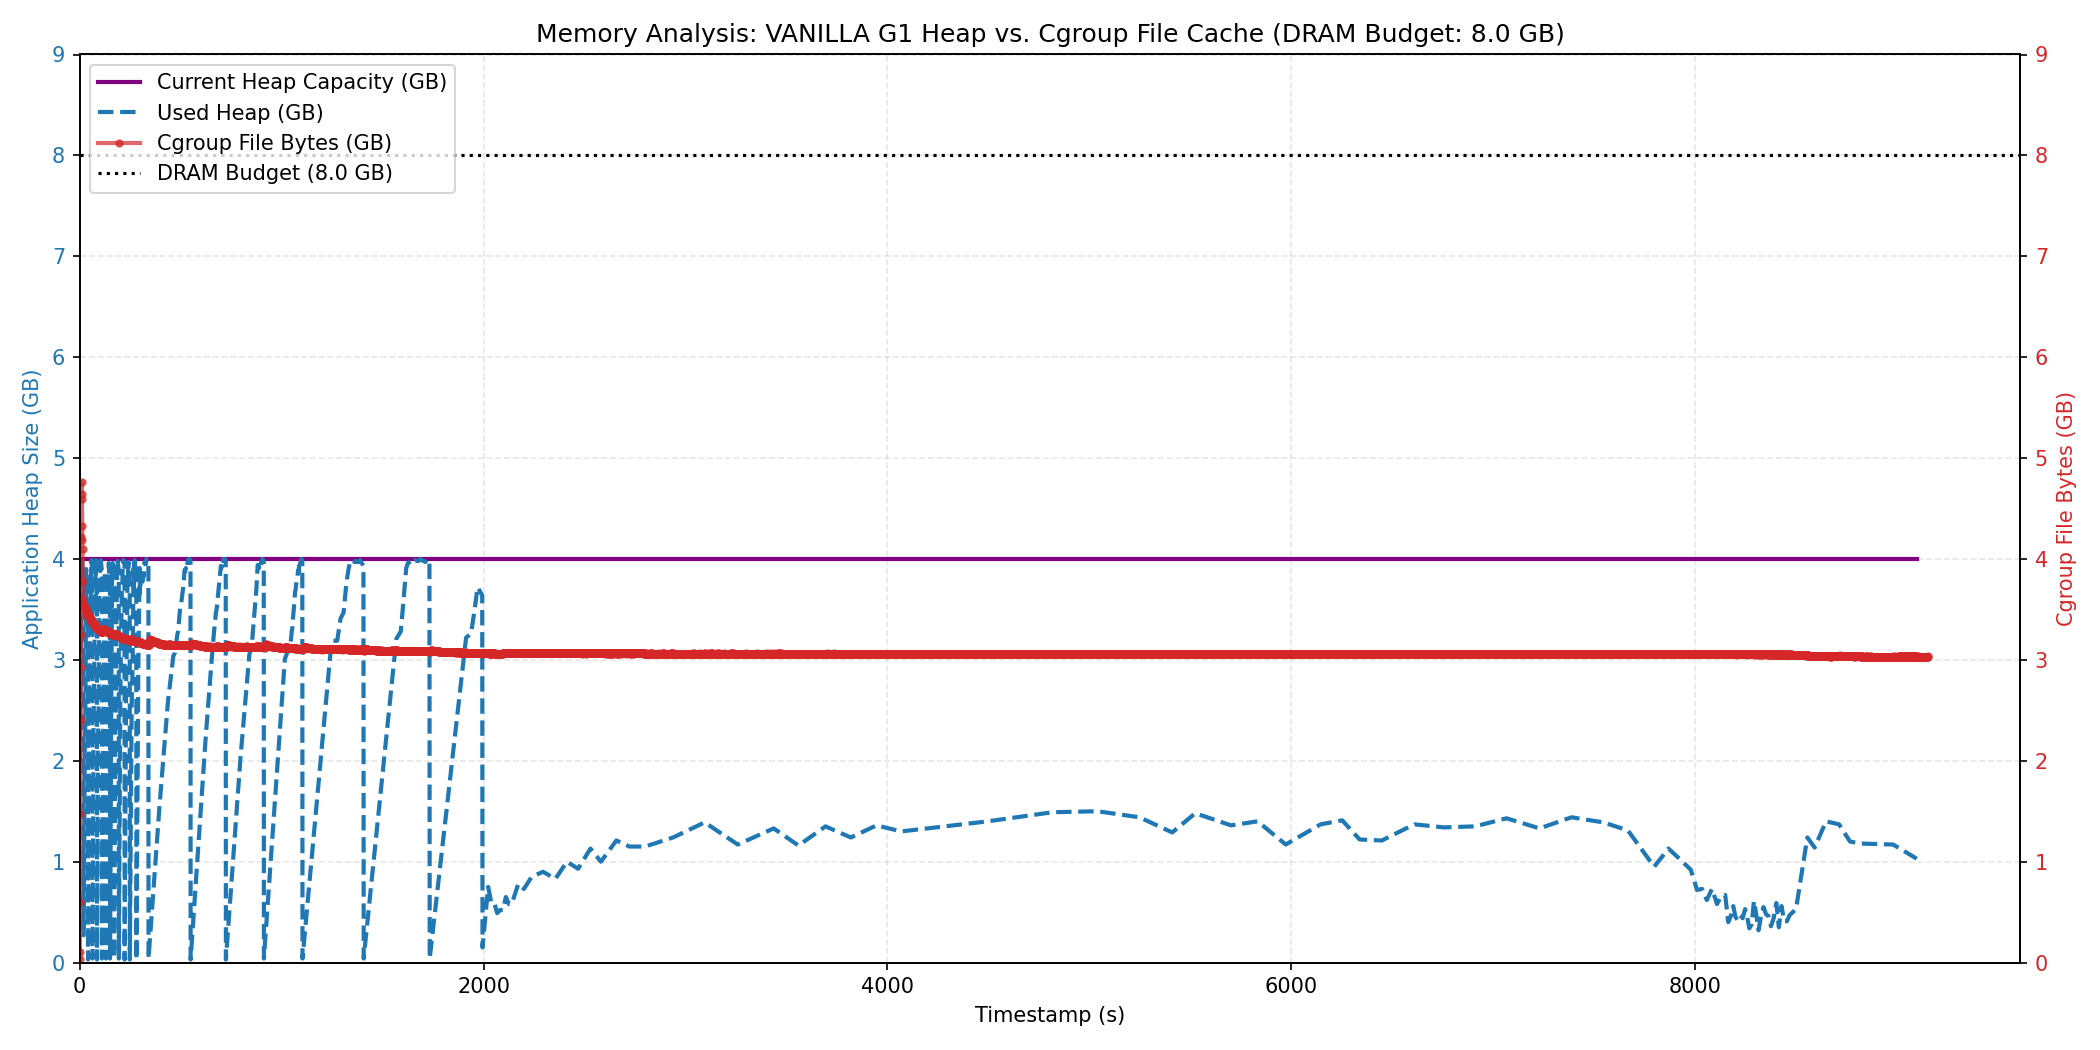
\includegraphics[width=1\linewidth]{fig/combined_memory_timeline_vanilla_g1.png}
	\caption{
		M1 Lucene benchmark with static DRAM configuration of 4GB H1 and 4GB pagecache.
	}
	\label{fig:vanilla-dram-underutilization}
\end{figure}

To address this limitation, we port \textbf{FlexHeap} \cite{flexheap} to our system, a dynamic
resizing policy that operates at runtime by dividing execution into sampling
intervals. During each interval, it tracks the number of CPU time consumed by Garbage-Collection (GC)
and the I/O overheads including I/O caused by accesses to
the (H2) memory-mapped file. At the end of each interval, it compares the
percent change between the two metrics, relative to the previous intervals. If
garbage collection overhead has increased more than I/O stalls, FlexHeap
signals G1 to grow the H1 heap to relieve GC pressure. Inversely, if I/O delays
have increased, a shrink heap action is invoked, shifting the remaining memory
towards the pagecache, via cgroups, to reduce evictions and hold more data from
the H2 file.

% \note{jk: write in which version of OpenJDK you have impement FlexHeap. Then
% 	discuss the high-level results}Across Lucene's and Spark's benchmarks, FlexHeap
% reports execution time improvements up to 70\% and 9\% accordingly.
%
% \note{jk: Here write in bullet points the contributions. For example, we show
% 	the problem of dynamic dram partitioning in tiered managed heaps. A second
% 	contibution is the implementation of FlexHeap on top of TeraHeap}

Across Lucene and Spark benchmarks, FlexHeap achieves 
execution time improvements of up to 70\% and 9\%, respectively, compared to 
TeraHeap with static DRAM partitioning. We implement FlexHeap as an extension 
to OpenJDK 17, extending TeraHeap.
In this thesis we make the following contributions:

\vspace{0.5em}
\begin{itemize}
\item We identify and analyze the limitations of static DRAM partitioning in a tiered managed heap 
  environment, highlighting how fixed memory allocations can not optimize performance 
  due to underutilized memory and I/O pressure.

\item We intergate \textbf{FlexHeap}, into G1 TeraHeap \cite{melidonis_thesis, mairh_thesis}

\item We evaluate FlexHeap on real-world Lucene and Spark workloads, showing consistent
  performance improvements and better DRAM utilization under certain memory budgets.

\end{itemize}

\section{Motivation}

\section{Design}

% eliminate bullets, make as paragraph

\subsection{Overview}

The goal of FlexHeap is to dynamically split DRAM between the primary heap (H1)
and the page cache used by TeraHeap’s secondary heap (H2), to reduce garbage
collection (GC) and I/O overheads. It monitors runtime behavior in short
intervals and uses a finite state machine (FSM) to decide when to grow or
shrink the main heap. GC and I/O costs are translated into lost CPU time and
then compared to determine the optimal resizing action. Expansion decisions are
scaled based on CPU usage and are bound between limits to prevent overly
aggressive or conservative heap growth. Shrink operations are more aggressive,
aiming to release memory back to the page cache by reclaiming up to 50\% of the
currently free heap regions. This design allows FlexHeap to respond to workload
changes and improve system performance dynamically.

% \subsection{Interval-Based Measurement Model}
\subsection{Estimating the impact of GC cost and I/O stalls}

All resizing decisions are made at the end of an interval. An interval is
defined as the time between two consecutive stop-the-world garbage collections
Young GCs, Mixed GCs or Full GCs). These intervals are recurring measurement windows in which both the
application threads (mutator) and the garbage collector (GC) can perform
working tasks. Within each interval, we estimate the cost of garbage collection and I/O activity,
to provide sufficient insight into system behavior to guide our dynamic resizing policy.
% \note{jk: our measurements are not accurate but they are an
% 	estimation of the costs. so you need to defind that we estimate the GC cost and
% 	I/O cost.}

During an interval, we track runtime metrics including:
\begin{itemize}
	\item The total CPU time lost due to GC, including stop-the-world pauses, concurrent GC threads, and refinement threads.
	\item The I/O overhead introduced by page cache while perfoming accesses to TeraHeap's secondary heap (H2).
\end{itemize}
	
\paragraph{Measuring STW pauses:} In these events
all application threads (mutators) are paused so that the JVM can exclusively perform
GC-related work. In order to calculate the time overheads produced by G1’s stop-the-world (STW) phases,
we measure the time spent inside key G1 safepoint functions.
Specifically we place timers around safepoint phases of the G1 garbage collector.
These include the stop-the-world pause for young and mixed collections, the concurrent
marking phase where the reachability of live objects is finalized and the full GC path
that reclaims the entire heap when necessary.

\paragraph{Measuring Concurrent GC threads:} These threads operate in the background,
concurrently with application execution.
Hence, in order to account for compute cycles lost to concurrent GC threads,
we must determine whether GC activity actually interferes with
application (mutator) execution. This interference only occurs when the combined number of
mutator threads and concurrent GC threads exceeds the number of available
CPU cores. In such cases, concurrent GC threads compete with the application
for CPU time, causing actual slowdown.

If the total mutator and GC threads is less or equal than the number of cores, the concurrent
GC threads are able to run on otherwise idle CPUs. In this case, we assume that
CPUs remaining idle do not cause performance loss.

Even under conditions where concurrent GC threads and mutator threads compete for CPU resources we avoid attributing all GC time as overhead.
We first subtract the amount of time GC threads could have used on idle cores estimated
as the number of free cores \texttt{\#cores} $-$ \texttt{\#mutators} $x$ \texttt{interval\_duration} .
The remaining time is treated as actual interference with the
application and is counted as GC overhead.

\paragraph{Measuring Refinement threads:} Refinement threads are a part of concurrent collection,
so the full runtime of refinement threads is interpreted as GC overhead. This is because refinement thread
activity directly supports concurrent GC phases and typically runs in the background,
contributing 100\% of their execution time to GC-related compute loss.


% \begin{itemize}
% 	\item \textbf{Measuring Stop-the-world (STW) pauses:} In these events
% 	      all application threads (mutators) are paused so that the JVM can exclusively perform
% 	      GC-related work. In order to calculate the time overheads produced by G1’s stop-the-world (STW) phases,
% 	      we measure the time spent inside key G1 safepoint functions.
% 	      Specifically we place timers around safepoint phases of the G1 garbage collector.
% 	      These include the stop-the-world pause for young and mixed collections, the concurrent
% 	      marking phase where the reachability of live objects is finalized and the full GC path
% 	      that reclaims the entire heap when necessary.
%
% 	      After obtaining the time spent in the safepoint functions, we translate it into CPU overhead, by using the following formula:
% 	      \[
% 		      \text{cpu\_time\_spent} += \text{gc\_pause\_time} \times \min(\text{mutators}, \text{cores})
% 	      \]
% 	      This formula estimates CPU cycles lost due to GC pauses by considering both the duration of the pauses and the level of available parallelism.
% 	      Although mutator threads are inactive during STW events, they represent potential application work that is delayed.
% 	      By only counting the threads that could actually run at the same time, we get a more accurate and realistic estimate of how much the application was slowed down.
%
% 	\item \textbf{Measuring Concurrent GC threads:} These threads operate in the background,
% 	      concurrently with application execution.
% 	      Hence, in order to account for compute cycles lost to concurrent GC threads,
% 	      we must determine whether GC activity actually interferes with
% 	      application (mutator) execution. This interference only occurs when the combined number of
% 	      mutator threads and concurrent GC threads exceeds the number of available
% 	      CPU cores. In such cases, concurrent GC threads compete with the application
% 	      for CPU time, causing actual slowdown.
%
% 	      If the total mutator and GC threads is less or equal than the number of cores, the concurrent
% 	      GC threads are able to run on otherwise idle CPUs. In this case, we assume that
% 	      CPUs remaining idle do not cause performance loss.
%
% 	      Even under conditions where concurrent GC threads and mutator threads compete for CPU resources we avoid attributing all GC time as overhead.
% 	      We first subtract the amount of time GC threads could have used on idle cores estimated
% 	      as the number of free cores \texttt{\#cores} $-$ \texttt{\#mutators} $x$ \texttt{interval\_duration} .
% 	      The remaining time is treated as actual interference with the
% 	      application and is counted as GC overhead.
%
% 	\item \textbf{Measuring Refinement threads:} Refinement threads are a part of concurrent collection,
% 	      so the full runtime of refinement threads is interpreted as GC overhead. This is because refinement thread
% 	      activity directly supports concurrent GC phases and typically runs in the background,
% 	      contributing 100\% of their execution time to GC-related compute loss.
%
% \end{itemize}

To measure garbage collection overhead, our system tracks the cumulative CPU time spent in each of these three components.
This data is collected in each interval and used by FlexHeap to determine whether GC-related costs are increasing or decreasing.

\subsubsection{I/O Monitoring via eBPF Library}  % make sub sub section

To accurately capture the I/O overhead produced by page‑cache accesses and
object transfers in the secondary heap (H2), we used an existing TeraHeap
eBPF‑based monitoring library. This library runs in kernel space and tracks
events such as page faults and read‑and‑write operations of mapped regions.
Whenever an object accessed in H2 triggers a page‑cache miss or eviction, the
library reports the data movement, which we convert into CPU‑equivalent lost
cycles. By integrating this eBPF library, I/O stalls can be translated into
equivalent CPU time lost, enabling a direct comparison with GC overheads during
each interval.

\subsection{Heap resizing decision making} % rename to somethging like decision making, or dram division...

Upon completion of an interval, FlexHeap collects the GC and I/O lost compute cycles and passes them through
a \textit{finite state machine (FSM)}. The FSM serves as a control mechanism
that reacts to both GC and I/O overhead percent changes and decides whether to adjust the DRAM allocation
between the heap (H1) and the page-cache. The FSM consists of 3 states:

Firstly, the \texttt{wait\_after\_grow} state, which represents a phase that occurs after
the system has increased the size of the heap (H1). Its purpose is to
to monitor whether the previous growth decision effectively
reduced overall overheads without destabilizing the system.

Each time the state is evaluated, FlexHeap retrieves runtime data from the G1 collector,
such as the current heap capacity, used and unused regions in bytes and the concurrent marking
start threshold (IHOP), to determine whether the heap is approaching
a GC initiation and whether there is available space for further expansions.

The decision logic follows several key checks:
\begin{itemize}
	\item If the total GC and I/O overhead has increased compared to the previous interval, the system
	      compares the relative growth rates of GC and I/O time. If GC overhead increased more than I/O,
	      FlexHeap interprets this as insufficient heap space and issues a \texttt{GROW\_HEAP} action,
	      provided the heap has not reached its maximum capacity.
	\item Conversely, if the I/O overhead increased more than the GC and the heap utilization is below 95\% of
	      total capacity, the system transitions to the \texttt{wait\_after\_shrink} state and issues a
	      \texttt{SHRINK\_HEAP} action, shrinking the heap and transferring DRAM to the page cache via cgroups.
	\item If none of these conditions are met, the system goes to a \texttt{no\_action\_state}.
\end{itemize}

Also, the systems uses IHOP as a safety condition. If the heap usage falls
below the IHOP limit and the current capacity is under the maximum allowed
size, the FSM remains in the grow state waiting to see if the system will
stabilize, without issuing any further grow actions.

The second state is the \texttt{wait\_after\_shrink}. Its purpose is to observe
how the system behaves after a heap shrinkage wihich consequently frees DRAM
back to the page cache. During this state, the FSM compares the garbage
collection (GC) with the I/O to determine whether the shrink operation had
reduced I/O pressure or, if further resizing actions are required.

The core logic of this state is as follows:
\begin{itemize}

	\item
	      If GC overhead have increased more than I/O, it indicates that shrinking the heap too aggressively,
	      led to increased GC activity. In this case, the system transitions to the \texttt{wait\_after\_grow} state
	      and performs a \texttt{GROW\_HEAP} action to give memory to the heap.

	\item If the I/O overhead increased the system stays in the \texttt{wait\_after\_shrink} state and issues further shrinks.
	      If the heap usage is still high (above 90\%), the FSM may also decide to grow again to relieve GC pressure.
\end{itemize}

Additionally, the state monitors total resident memory (rss) and page cache
usage. If the sum of resident memory and page cache usage falls below 80\% of
the configured DRAM limit, the FSM interprets is as (\texttt{IOSLACK}) and
issues another \texttt{SHRINK\_HEAP} action to allocate more memory to the page
cache. This allows to reclaim unused DRAM to relieve I/O when the system is
under light memory pressure.

If none of these conditions are triggered, the FSM
transitions to \texttt{no\_action}.

At last the FSM supports the \texttt{no\_action} state, which is the default state.
When the system enters this state, no DRAM resizing actions were performed.

At each interval, FlexHeap evaluates whether the total GC and I/O time has
changed. If the change is within a 5\% threshold, it is interpreted
as noise or a stable condition and the system remains in the \texttt{no\_action} state.

If the combined overhead has increased notably and the system is in this state, the FSM analyzes which overhead (GC or I/O) is
contributing more to the increase:
\begin{itemize}
	\item If the GC overhead has increased more than I/O, this suggests that H1 may need a grow action.
	      In that case, FlexHeap transitions to the \texttt{wait\_after\_grow} state and issues a \texttt{GROW\_HEAP} action,
	      unless the heap has already reached its maximum capacity.

	\item If the I/O overhead has increased more, FlexHeap checks if the heap usage is above 90\% of
	      its capacity. If not, the system transitions to \texttt{wait\_after\_shrink} and issues a \texttt{SHRINK\_HEAP}
	      action to return DRAM to the page cache.
\end{itemize}

If the total overhead has decreased compared to the previous interval, no resizing action is needed. In this case,
the system remains in the \texttt{no\_action} state.

\subsection{Heap Resizing Step}

When an expansion is required, the system calculates, by using the vanilla-G1's
resizing step, how much uncommitted memory is available. This is the memory
that has been reserved by the JVM but not yet used. A scaling factor is
computed based on the change in CPU overhead compared to the previous
measurement interval. This factor determines the aggressiveness of the heap
expansion and is bounded to prevent overly conservative or excessively
aggressive resizing. The final resize amount is then clamped within threshold
values to ensure it stays within bounds, large enough to make a adjustments,
but not to exhaust the remaining memory and create GC pressure.

In contrast, shrink decisions are more aggressive. Since returning DRAM to the
operating system's page cache can significantly reduce I/O delays for TeraHeap
workloads, shrink operations prioritize releasing unused memory. The amount of
memory to shrink is derived from the number of free heap regions—memory that
has already been committed but is not actively in use. A fixed scaling factor
(50\%), is then applied to determine how much of the free memory can be
reclaimed, ensuring that the main heap retains sufficient headroom for sudden
bursts of memory allocation without triggering excessive garbage collection.


\section{Methodology}

Using FlexHeap, we perform a series of experiments to evaluate: 
(1) how FlexHeap compares to the baseline TeraHeap system without dynamic heap resizing,
(2) the impact of dynamic resizing on garbage collection overhead and
(3) the reduction in I/O traffic to the secondary heap device (H2).
These metrics allow us to assess both runtime performance and DRAM utilization efficiency.

Our experiments run on a high-performance dual-socket Intel server.
The system is equipped with two Intel Xeon Gold 5318Y CPUs, each with 24 physical cores 
and 2 hardware threads per core, for a total of 96 logical CPUs. It includes 256\,GiB of DRAM 
distributed across four NUMA nodes, with swap disabled. We co-locate all threads on a single
NUMA node to eliminate NUMA interference and use Linux cgroups to restrict the available DRAM,
enabling controlled and memory-constrained experiments.

For storage, we used two high-speed NVMe SSDs and one large-capacity SATA disk:
\begin{itemize}
  \item \texttt{/dev/nvme1n1}: a 1.8\,TB device formatted with \texttt{XFS}, used as the location of 
                               the H2 heap file for both Lucene and Spark workloads.
  \item \texttt{/dev/nvme2n1}: a 1.9\,TB device (\texttt{XFS}), used as the dataset disk for Lucene 
                               and the shuffle directory for Spark.
  \item \texttt{/dev/sda1}: a 3.6\,TB \texttt{EXT4} disk, used to store the Spark dataset.
\end{itemize}

All storage devices are directly attached with no RAID configuration. The operating system is Ubuntu 
24.04.1\,LTS with a Linux kernel version\,6.8.0-1020-nvidia.
\subsection{Lucene Methodology}

We evaluate our system using a real-world 200\,G Lucene index containing 52.6 billion words. 
To support the second-tier heap (H2), we preallocate a 300\,G file on NVMe storage, which serves as space 
for the query-cache to reside.
The dataset is preprocessed by removing stop words, single-character tokens, and non-English words. 
Terms are then grouped by frequency into two categories: high-frequency (top 1\%) and medium-frequency. 
High-frequency terms dominate document access patterns and generate significantly more I/O pressure.


We define two workloads:
\begin{itemize}[leftmargin=1.5em]
  \item \textbf{M1}: high-frequency small queries retrieving the top 50 results.
  \item \textbf{M2}: high-frequency large queries retrieving up to 500{,}000 results.
\end{itemize}

We run both M1 and M2 workloads under four DRAM budgets: 40\,G, 20\,G, 10\,G, and 8\,G,
enforced using Linux cgroups to control memory. 
For each DRAM setting, we evaluate both the static and a dynamic heap configuration. 
The static configuration, \textbf{TeraHeap}, evenly partitions the available DRAM between the 
managed heap (H1) and the page cache (H2), allocating 50\% of memory to each. In contrast, 
the dynamic configuration uses the \textbf{FlexHeap} policy, which adjusts the size of H1 
at runtime based on application behavior, while reserving a fixed 2\,GiB of DRAM for the page cache across all runs.

This setup allows us to evaluate the benefits of dynamic heap resizing under different memory constraints and workload pressures. 
The main heap (H1) sizes for different DRAM configurations are presented in Table~\ref{tab:lucene-configs}.

% \begin{table}[H]
% \centering
% \renewcommand{\arraystretch}{1.3}
% \caption{Lucene configurations for workloads M1 and M2 under.}
% \label{tab:lucene-configs}
% \begin{tabular}{|l|c|c|}
% \hline
% \textbf{Configuration} & \textbf{DRAM Budget} & \textbf{H1 / H2 Allocation (GiB)} \\
% \hline
% \multirow{4}{*}{TeraHeap (static)} 
%                        & 40\,G             & 20\,G / 20\,G \\
%                        & 20\,G             & 10\,G / 10\,G \\
%                        & 10\,G             & 5\,G / 5\,G   \\
%                        & 8\,G              & 4\,G / 4\,G   \\
% \hline
% \multirow{4}{*}{FlexHeap (dynamic)} 
%                        & 40\,G             & 38\,G / 2\,G  \\
%                        & 20\,G             & 18\,G / 2\,G  \\
%                        & 10\,G             & 8\,G / 2\,G   \\
%                        & 8\,G              & 6\,G / 2\,G   \\
% \hline
% \end{tabular}
% \end{table}

\begin{table}[H]
\centering
\renewcommand{\arraystretch}{1.1}
\caption{Lucene H1 size configurations for workloads M1 and M2.}
\label{tab:lucene-configs}
\begin{tabular}{|l|c|c|c|c|}

\hline
  \textbf{DRAM Budget} & 40\,G & 20\,G & 10\,G & 8\,G \\
\hline
  TeraHeap (static)& 20\,G & 10\,G & 5\,G & 4\,G \\
\hline
  FlexHeap (dynamic)& 38\,G & 18\,G  & 8\,G & 6\,G \\
\hline
 
\end{tabular}
\end{table}

\subsection{Spark Methodology}
\label{sec:spark-methodology}

We evaluate our dynamic heap resizing mechanism using a set of Spark workloads 
from the \texttt{spark-bench} suite. The selected benchmarks consist of:
(\texttt{PageRank}, \texttt{ConnectedComponent}, \texttt{ShortestPaths}, \texttt{TriangleCount}) 
and machine learning tasks (\texttt{SVDPlusPlus}, \texttt{LinearRegression}, \texttt{LogisticRegression}).

Similarly to Lucene, in the \textbf{TeraHeap} setup, the DRAM is partitioned statically between the managed heap (H1) and the second-tier 
storage-backed heap (H2), with allocation ratios manually chosen for each individual workload. In contrast, \textbf{FlexHeap} 
dynamically adjusts the size of H1 during execution, reserving part of the available DRAM for the page cache depending on
the runtime requirements of each benchmark. 

The total DRAM budget is workload-specific and chosen for each benchmark.
The heap allocations for both TeraHeap and FlexHeap configurations are summarized in Table~\ref{tab:spark-benchmark-configs}.
This setup enables us to evaluate how static versus dynamic DRAM partitioning impacts performance across different Spark tasks.


\begin{table}[H]
\centering
\small
\renewcommand{\arraystretch}{1}
\caption{Spark benchmark configurations under TeraHeap (static) and FlexHeap (dynamic).}
\label{tab:spark-benchmark-configs}
\begin{tabular}{|l|l|c|}
\hline
\textbf{Configuration} & \textbf{Benchmark} & \textbf{H1/ H2 Allocation (G)} \\
\hline
\multirow{7}{*}{TeraHeap (static)} 
& PageRank             & 64\,G / 16\,G \\
& ConnectedComponent   & 68\,G / 16\,G \\
& ShortestPaths        & 48\,G / 16\,G \\
& TriangleCount        & 64\,G / 16\,G \\
& SVDPlusPlus          & 24\,G / 16\,G \\
& LinearRegression     & 54\,G / 16\,G \\
& LogisticRegression   & 54\,G / 16\,G \\
\hline
\multirow{7}{*}{FlexHeap (dynamic)} 
& PageRank             & 74\,G / 6\,G  \\
& ConnectedComponent   & 80\,G / 4\,G  \\
& ShortestPaths        & 48\,G / 16\,G \\
& TriangleCount        & 64\,G / 16\,G \\
& SVDPlusPlus          & 28\,G / 12\,G \\
& LinearRegression     & 64\,G / 6\,G  \\
& LogisticRegression   & 60\,G / 10\,G \\
\hline
\end{tabular}
\end{table}

%
% \begin{table*}[!t]
% % \begin{table}[!htbp]
% % \begin{center}
% \renewcommand{\arraystretch}{1.3}
% \resizebox{\textwidth}{!}{%
% \begin{tabular}{|l|c|c|c|c|c|c|c|}
% \hline
% \textbf{Configuration} & \textbf{PageRank} & \textbf{ConnectedComponent} & \textbf{ShortestPaths} & \textbf{TriangleCount} & \textbf{SVDPlusPlus} & \textbf{LinearRegression} & \textbf{LogisticRegression} \\
% \hline
% TeraHeap (static DRAM) & 64G H1 / 16G H2 & 68G H1 / 16G H2 & 68G H1 / 16G H2 & 64G H1 / 16G H2 & 24G H1 / 16G H2 & 54G H1 / 16G H2 & 54G H1 / 16G H2 \\
% \hline
% FlexHeap               & 74G H1 / 6G H2  & 80G H1 / 4G H2  & 48G H1 / 10G H2 & 64G H1 / 16G H2 & 28G H1/ 12G H2 & 64G H1/ 6G H2 & 60G H1/ 10G H2  \\
% \hline
% \end{tabular}
% }
% \caption{Spark benchmarks under two configurations: TeraHeap with static DRAM partitioning and FlexHeap.}
% \label{tab:spark-benchmark-configs}
% % \end{center}
% \end{table*}
% \vspace{-1em}  % optional: reduce whitespace
%



\section{Evaluation}
\subsection{Dynamic Heap Resizer vs Static DRAM configurations}
First, we investigate the performance of Dynamic Heap Resizer 
(DHR) compared to two static configurations: (1) hand-tuned 
(ideal) and (2) even DRAM division (50-50). 
Figure~\ref{fig:gc_exec_time} depicts the normalized 
execution time of three representative Lucene benchmarks 
(M1, M2, and M3) on the Titan2 server. Within each group,
the first and second columns correspond to static ideal and 
static 50-50 partitioning, respectively, while the third
column represents DHR.

Overall, DHR consistently outperforms both static
configurations across all benchmarks. In particular,
compared to the static 50-50 configuration (even), DHR
achieves execution time reductions of 14.3\% for M1, 15.8\% 
for M2, and 1.3\% for M3. Compared to the hand-tuned (ideal)
configurations, DHR provides performance improvements of 
up to 13.4\% (M2). 
Although DHR improves overall performance, we observe an increase 
in GC time, particularly in M1 and M2. This increase is attributed
to high minor GC activity caused by the creation of many backward 
pointers within these workloads. Backward pointers are references 
from older to younger objects, which prevent objects from being 
collected during minor GCs, resulting in higher promotion rates and
increased GC overhead.

Specifically, GC time nearly doubles in M1 (1.87–1.93× increase) and
increases by approximately 19\% (1.18×) in M2 compared to static configurations. 
In contrast, M3 exhibits a slight decrease in GC time, indicating minimal backward 
pointer impact.


\begin{figure}[htbp]
  \centering
  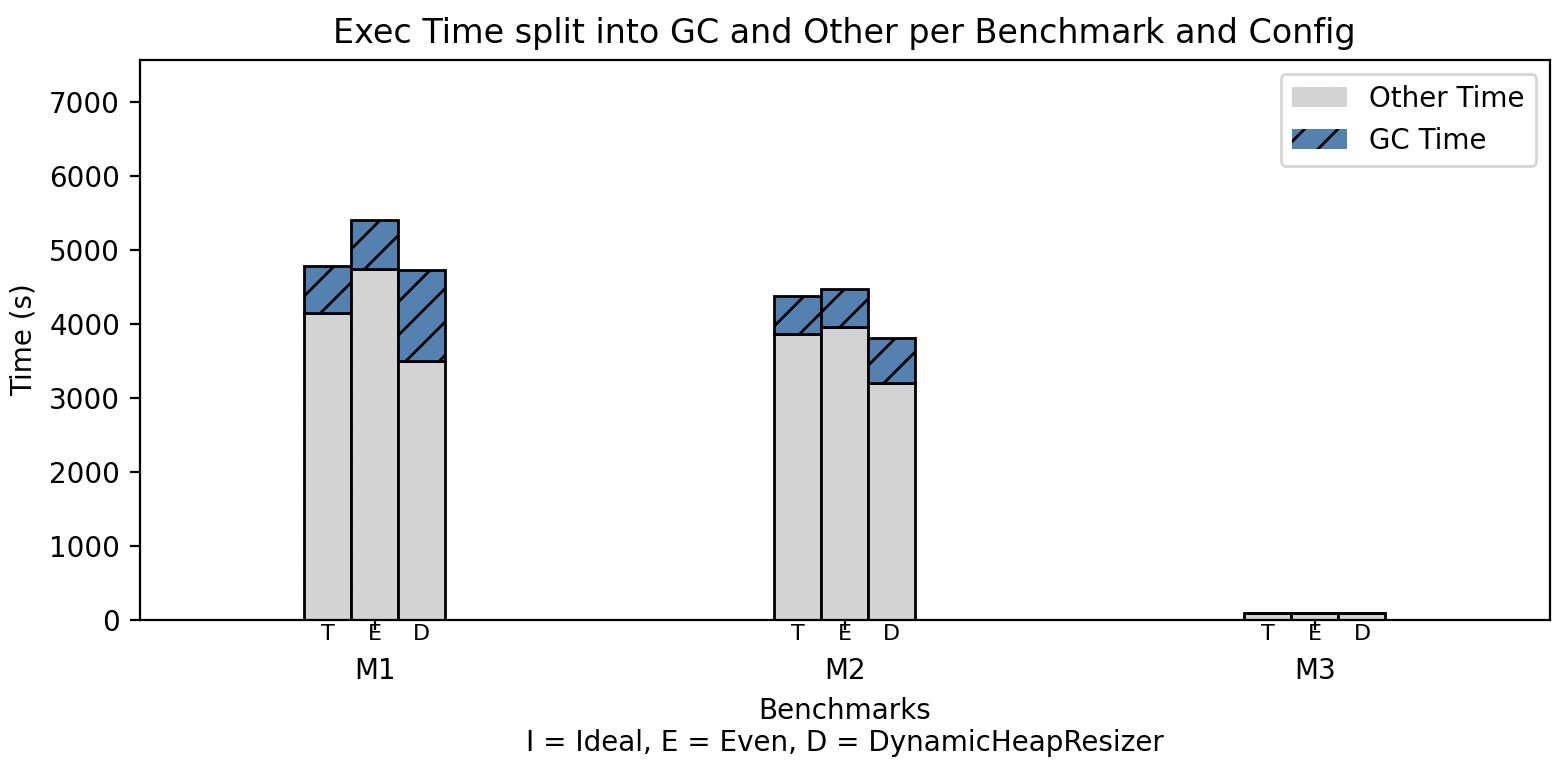
\includegraphics[width=1\columnwidth]{fig/eval_graph.png}
  \caption{Execution time and GC time comparisons}
  \label{fig:gc_exec_time}
\end{figure}

\subsection{Page Cache Usage and Device Traffic}

In this subsection, we analyze the page cache utilization under the Dynamic Heap Resizer
(DHR) for the three evaluated workloads: M1, M2, and M3. Figure~\ref{fig:pc_dhr} 
illustrates the page cache usage over time demonstrates different caching behaviors, 
adapting to each benchmark and their distinct memory access patterns and working set sizes.

For M1, the page cache usage increases rapidly during the initial phase of execution, 
stabilizing at approximately 17.6~GB. This indicates that M1 aggressively utilizes 
the page cache early on, due to frequent and repeated accesses.
After the initial rise, the flat line shows that M1's data fits in the page cache, so later accesses have less I/O delay.
M2, exhibits a more gradual increase in page cache usage, 
eventually reaching a similar final usage level of around 17.5~GB.
This slower increase is due to the workload consisting of more distributed 
data accesses, taking longer to populate the page cache fully. This 
indicates that M2 patterns require more time to reach an optimal cache utilization.
M3 shows periodic drops and rises, indicating batching behavior with bursts of cache usage between processing phases.

Overall, these results indicate that the Dynamic Heap Resizer effectively manages DRAM allocation to maximize page
cache utility for workloads that benefit from dynamic partitioning at runtime. 

\begin{figure}[htbp]
  \centering
  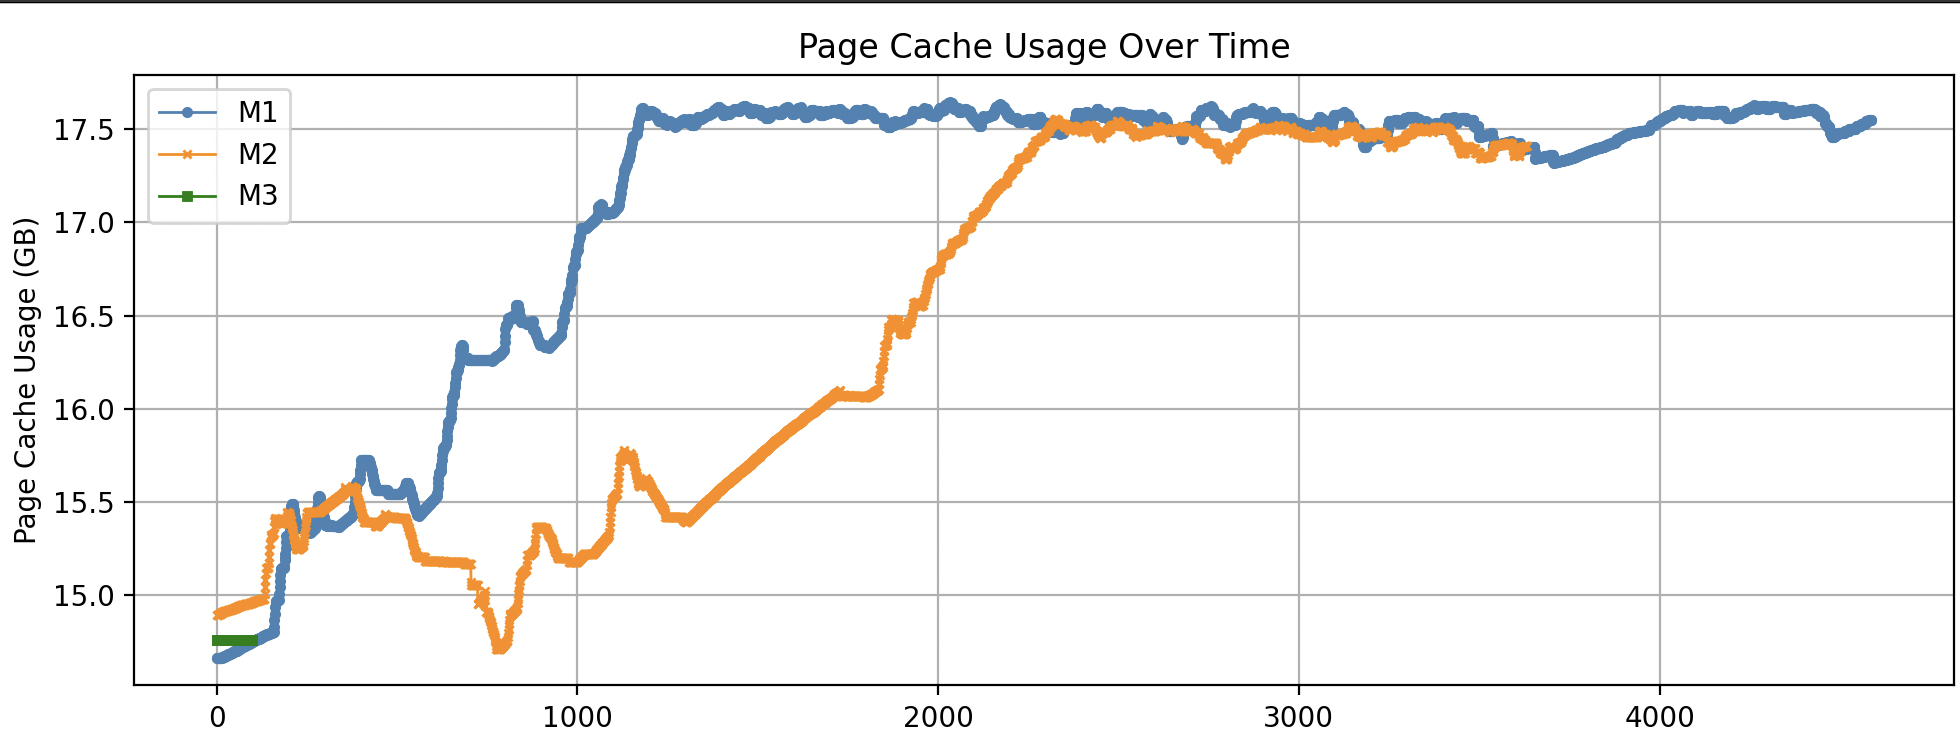
\includegraphics[width=1\columnwidth]{fig/pagecache_dhr.png}
  \caption{Page cache usage with Dynamic Heap Resizing, for M1, M2, M3 benchmarks}
  \label{fig:pc_dhr}
\end{figure}

\begin{table}[h]
\centering
\caption{Average read and write traffic (MB/s) for each benchmark under Ideal, Even, and DHR configurations.}
\label{tab:traffic}
\begin{tabular}{l|ccc|ccc}
\hline
 & \multicolumn{3}{c|}{Read (MB/s)} & \multicolumn{3}{c}{Write (MB/s)} \\
Config & M1 & M2 & M3 & M1 & M2 & M3 \\
\hline
Ideal & 0.07 & 0.07 & 0.002 & 22.79 & 22.59 & 0.01 \\
Even  & 0.07 & 0.07 & 0.002 & 20.80 & 21.24 & 0.01 \\
DHR   & 0.07 & 0.08 & 0.002 & 24.80 & 28.06 & 0.05 \\
\hline
\end{tabular}
\end{table}

\subsection{Query Throughput (QPS) Analysis}

Figure~\ref{fig:qps_plot}: Compares Queries per second (QPS) for each benchmark (M1, M2, M3)
under Ideal, Even, and Dynamic Heap Resizer (DHR) configurations.

In this plot, we observe that for M1, DHR achieves the highest QPS compared to both 
Ideal and Even configurations, indicating that dynamically adapting the heap provides
benefits for this workload. For M2, DHR again slightly outperforms both Ideal and Even, 
showing that its adjustments handle the memory and I/O requirements effectively. In M3,
however, DHR achieves slightly lower QPS compared to Ideal, but remains higher than the
Even configuration. This minor difference suggests that the Dynamic Heap Resizer’s gradual 
adjustments cannot resize aggressively enough during batched phases.
Overall, DHR shows improved or comparable QPS across benchmarks, demonstrating its ability 
to adapt efficiently to varying workload characteristics.

\begin{figure}[htbp]
  \centering
  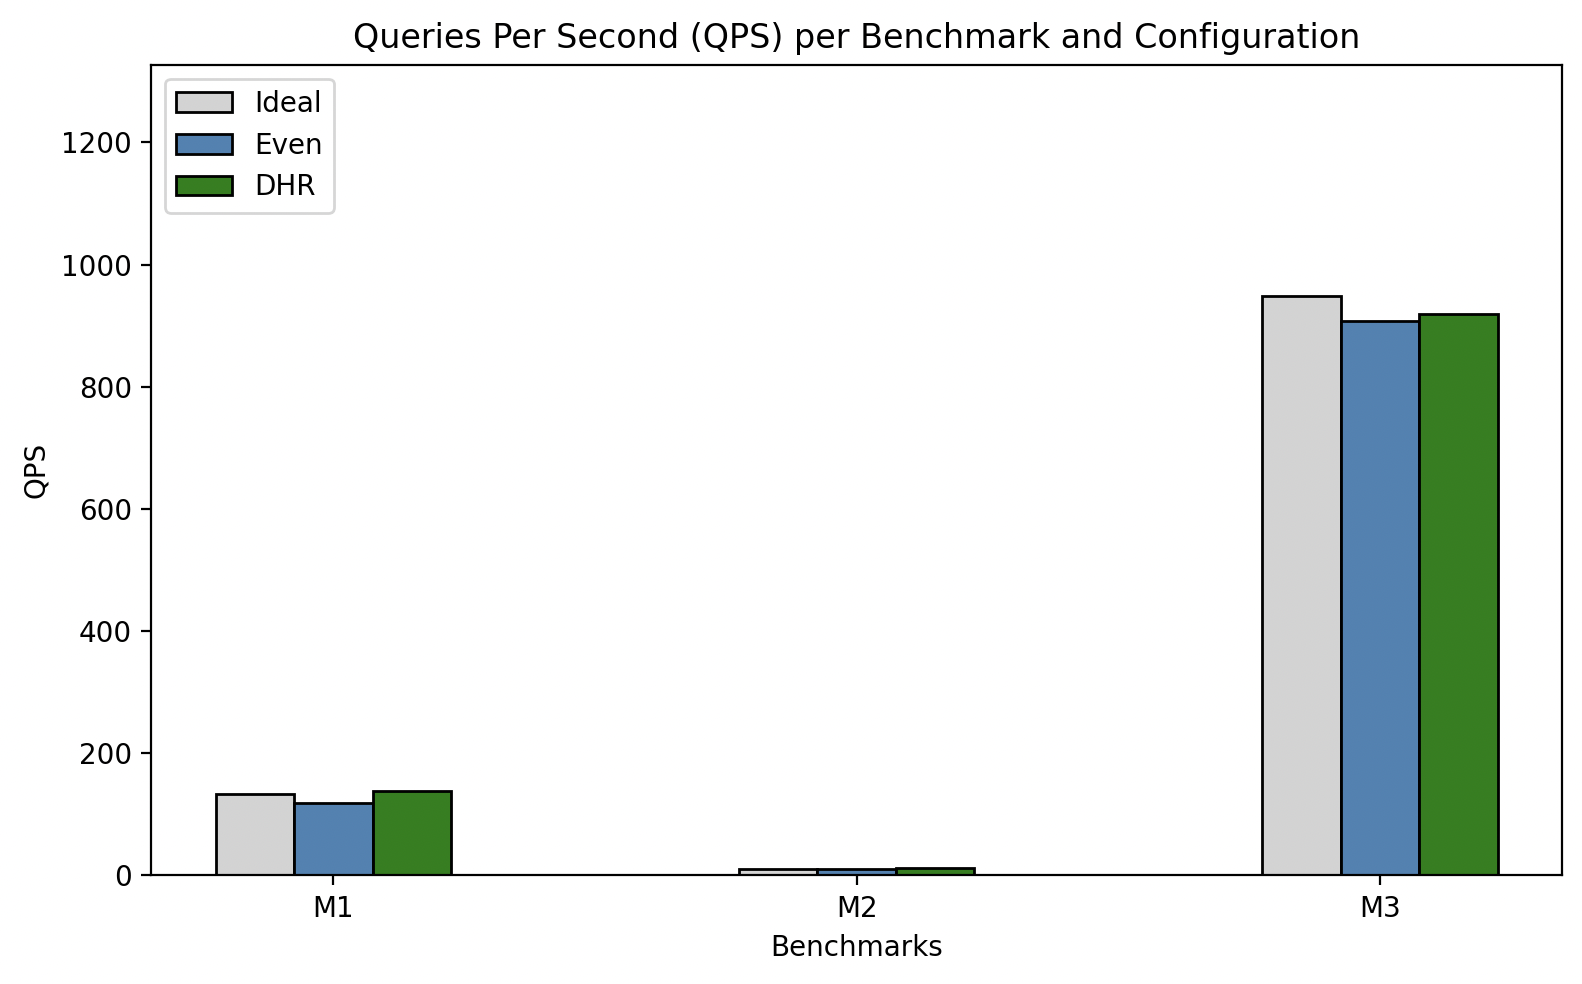
\includegraphics[width=1\columnwidth]{fig/qps_plot.png}
  \caption{Queries per second (QPS) for benchmarks M1, M2, and M3}
  \label{fig:qps_plot}
\end{figure}


\section{Related Work}
Prior approaches fall into four categories: cached heaps, tiered heaps, hybrid heaps, and managed heap resizing techniques.

Cached heaps like Semeru \cite{semeru}, MemLiner \cite{memliner}, and Mako \cite{mako} allocate the managed heap entirely on remote memory while using local DRAM as a cache. These systems often require kernel modifications to implement remote paging and suffer from high I/O traffic and GC overheads due to frequent object scans and evacuations between memory tiers. For example, Semeru offloads GC scans to remote JVM instances to mitigate latency, while MemLiner reorganizes GC thread memory access order to align with mutator access patterns. However, both still suffer from costly object transfers and rewriting between memory tiers. Mako further introduces a Heap Indirection Table to track object locations, which imposes load reference barriers on every access, adding CPU overhead. Friendly-NVM-GC \cite{friendlynvmgc} uses DRAM as a cache for a heap entirely placed on NVM but cannot avoid slow GC scans over NVM-resident objects.

Tiered heaps aim to reduce write amplification or NVM access latencies. Crystal Gazer \cite{crystalgazer1, crystalgazer2} and GCMove \cite{gcmove} frequently migrate objects between DRAM and NVM generations to limit writes but incur slow scans to update references. ThinGC \cite{thingc} ensures mutators never directly access NVM-resident objects by moving them into DRAM upon access, avoiding immediate reference updates through lazy barriers, but this increases DRAM memory pressure and GC frequency. JPDHeap \cite{jpdheap} requires programmers to annotate objects for placement across DRAM and NVM, again leading to expensive NVM scans for reference adjustments.

Hybrid heaps such as Melt \cite{melt} and LeakSurvivor \cite{leaksurvivor} place hot objects in DRAM and cold objects on HDD or SSD, maintaining a user-space cache inside the JVM to track object offsets. While effective for HDD latency, they require a cache lookup for every access, adding CPU management overhead. TeraHeap \cite{TeraHeap}, on the other hand, targets NVMe SSDs with memory-mapped I/O to reduce cache lookup costs, but its DRAM partition between the heap (H1) and page cache for the secondary heap (H2) is statically configured and does not adapt to workload changes.

Finally, managed heap resizing techniques focus on improving GC performance by dynamically adjusting heap sizes. Brecht et al. \cite{brecht} propose aggressive heap expansion in Boehm GC to reduce execution time, while Yang et al. \cite{yang} develop an analytical model for heap resizing in multi-tenant environments. ElasticMem \cite{elasticmem} reclaims heap memory for other processes in shared clusters to increase throughput. White et al. \cite{white} use PID controllers to meet user-defined GC goals by tuning heap resize ratios. However, these approaches solely optimize GC behavior without considering I/O costs, limiting their applicability to hybrid heaps that require balanced DRAM allocation between managed memory and page cache for performance stability.

In contrast to these systems, our Dynamic Heap Resizer monitors runtime GC overhead and I/O cost, enabling dynamic partitioning of DRAM within hybrid managed heaps.

\section{Conclusions}
In modern hybrid heap setups, large-scale search engines such as 
Lucene exhibit dynamic variations in memory requirements between 
the DRAM-managed heap and the I/O cache. The conventional approach of statically dividing DRAM
between these two tiers is inadequate for addressing such demands, 
leading to performance bottlenecks. In this
work, we propose and evaluate the Dynamic Heap Resizer, a lightweight runtime
mechanism that continuously reallocates DRAM between the managed heap and the
H2 page cache based on GC and I/O costs. Our evaluation on representative Lucene
query workloads demonstrates that the Dynamic Heap Resizer adapts efficiently 
to changing memory and I/O patterns, improving execution time by up to 15.8\% 
compared to static 50-50 partitioning and 13.4\% compared to the ideal configurations, without requiring manual tuning. Overall, 
dynamic memory resizing offers an effective solution to to reduce the execution time 
of Lucene under constrained DRAM budgets.





\bibliographystyle{plain}
\bibliography{paper}

%-------------------------------------------------------------------------------
\end{document}
%-------------------------------------------------------------------------------
